\chapter{Introduction}\label{intro}

Ce chapitre présente dans un premier temps le type d'architecture employé (cf. \ref{intro.archi}) 
pour organiser le code source et décrit ensuite les différents chapitres de ce document 
(cf. \ref{intro.chapitrage}). Dans un second temps, ce chapitre récapitule aussi brièvement les 
langages utilisés (cf. \ref{intro.langages}) et ainsi que les sous-dossiers qui structurent le 
code source (cf. \ref{intro.folders}).

\section{Architecture générale}\label{intro.archi}

La conception de PAG applique l'architecture 
\textbf{MVC}~\footnote{Cf. \url{https://fr.wikipedia.org/wiki/MVC}}, 
c.-à-d. \textit{\underline{M}odèle - \underline{V}ue - \underline{C}ontrôleur}, illustrée à 
la figure~\ref{fig.concept.MVC}. Cette architecture 
vise à séparer clairement le code qui va représenter les données (le modèle), le code qui va 
fournir une interface à l'utilisateur (la vue) et le code qui va gérer la logique des opérations 
réalisées par l'utilisateur (le contrôleur).

\vspace{-0.2cm}
\begin{center}
    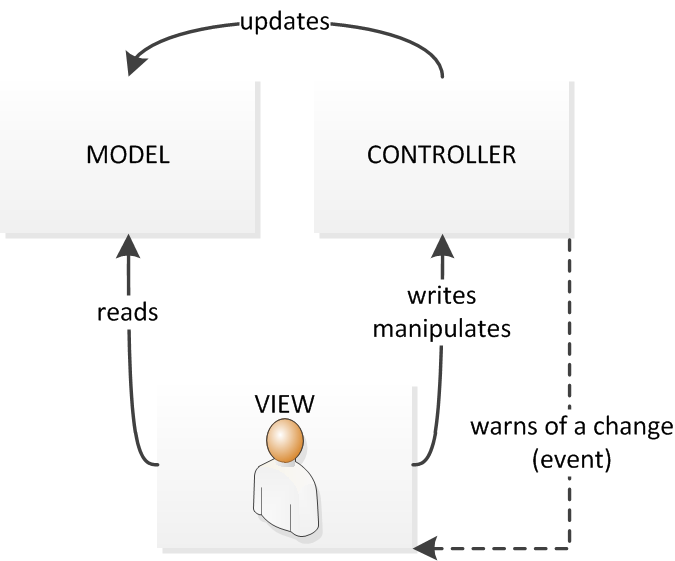
\includegraphics[scale=1.0]{figures/ModeleMVC.png}
	\captionof{figure}{Vue conceptuelle du \textit{design pattern} MVC (source: Wikipédia)}
	\label{fig.concept.MVC}
\end{center}
\vspace{-0.2cm}

Dans le cas de PAG, en pratique, le modèle rassemble un ensemble de classes PHP qui vont servir 
d'abstraction pour le contenu de la base de données, tandis que la vue est constituée d'une part 
d'un ensemble de sous-dossiers qui vont isoler les fichiers écrits dans certains langages (ici, 
le CSS et le JavaScript) et d'autre part d'un ensemble de \textit{templates} et % TODO: ref vers un autre chapitre 
de fonctions d'interprétation intermédiaire qui vont isoler le code HTML et son agencement selon 
l'utilisateur du reste. Les scripts principaux, écrits en PHP et situés majoritairement à la 
racine du site, s'apparentent à la partie contrôle et se veulent le plus haut niveau possible 
(c.-à-d., en reléguant les aspects plus techniques à d'autres parties du code). Notez qu'un 
détail des sous-dossiers est donné à la section~\ref{intro.folders}.

En pratique, cela veut dire que les scripts principaux (écrits en PHP)
\begin{itemize}
\item ne contiennent aucune requête directe vers la base de données, et mentionnent tout au plus 
les débuts et les fins de transactions avec celle-ci (c.-à-d. une suite logique d'interactions 
qu'on doit pouvoir annuler si l'une d'entre elles échoue et compromet l'intégrité des données), 
\item ne comportent pas ou peu de CSS (langage utilisé pour coder le style visuel) ou de 
JavaScript (langage utilisé pour coder les interactions), se contentant de lister les fichiers 
écrits dans ces langages qui seront utilisés pour créer le rendu de la page finale et gérer 
son interactivité, 
\item ne comportent pas non plus de HTML (langage utilisé pour structurer une page Web) ou très 
peu, celui-ci étant écrit pour la majeure partie dans des \textit{templates} isolés dans la 
partie \textit{vue} du code.
\end{itemize}
\vspace{0.3cm}

Il ne reste alors que la logique "\textit{haut-niveau}" qui va régir les actions de l'utilisateur. 
Pouvoir isoler cette logique du reste du code est très important pour sa lisibilité: comme les 
lecteurs du code pourront s'en apercevoir, certaines pages manipulent plusieurs fonctionnalités 
(assez souvent optionnelles) d'un coup. S'il est tout à fait possible de reproduire tout un script 
en mélangeant tout à la fois les différents langages utilisés (cf. \ref{intro.langages}), 
le résultat serait beaucoup plus verbeux et confus à la lecture.

\section{Contenu de ce document}\label{intro.chapitrage}

Le but de ce document est de présenter les grandes lignes du code source en allant progressivement 
du modèle (le \underline{M} de MVC) vers le contrôleur (le \underline{C}), ou plus exactement vers 
les scripts PHP "en pratique", c.-à-d. ceux qui décrivent le comportement de chaque page du site 
tout en minimisant les détails techniques.

Le chapitre~\ref{headerlib} commence par présenter la librairie d'en-tête \texttt{Header.lib.php} 
(située dans le sous-dossier \texttt{libraries/}) qui fournit plusieurs classes~\footnote{En 
écrivant ce document, je suppose que le lecteur est déjà familier avec la programmation 
orientée-objet. Des tutoriels pour son utilisation en PHP peuvent être facilement trouvés sur le 
Web.} statiques servant de base commune à l'ensemble des scripts PHP. Connaître celles-ci et leur 
utilité est indispensable pour bien comprendre le reste du code. Ces classes incluent notamment la 
gestion de la connexion à la base de données (et les interactions avec celle-ci) ainsi que la 
gestion de la connexion de l'utilisateur sous un pseudonyme.

Ensuite, le chapitre~\ref{model} présente le \textit{Modèle}, c.-à-d. l'ensemble des classes PHP 
utilisées pour manipuler sous forme d'objets les données du site (par exemple les utilisateurs, 
les sujets, les messages qu'ils contiennent, etc.) telles que stockées dans la base de données. La 
conception de ces classes vise en particulier à isoler les requêtes SQL (le langage utilisé pour 
dialoguer avec la base de données) liées à la manipulation des données (insertion, lecture ou 
modification de lignes dans la base de données) du reste du code.

Le chapitre~\ref{view} décrit ensuite la \textit{Vue}, c.-à-d. comment les données sont traitées 
afin de produire une page web affichable. Cette "traduction" des données se fait principalement 
à l'aide d'un moteur de \textit{templates} fait maison, mais pour certains éléments du site dont 
l'affichage peut dépendre des préférences et des interactions de l'utilisateur, des 
\textit{représentations intermédiaires} (dans le code source, \textit{IR} pour 
\textit{\underline{I}ntermediate \underline{R}epresentation}) traduisent les données brutes en un 
format plus adapté au moteur de templates.

Enfin, le chapitre~\ref{control} présente les grandes lignes des scripts principaux (c.-à-d. la 
partie \textit{Contrôle} du code), c.-à-d. comment les différents composants vus dans les 3 
chapitres antérieurs sont manipulés pour créer des scripts "haut niveau" qui implémentent les 
comportements voulus tout en minimisant le mieux possible les détails techniques.

Notez que des sections annexes existent sous forme de chapitre~\ref{annexes} et fournissent 
quelques justifications quant à certains choix qui ne tiennent pas de l'implémentation.

\section{Langages utilisés}\label{intro.langages}

Le code de PAG fait intervenir 5 langages différents couramment utilisés dans le développement 
web. Pour les lecteurs moins familiers avec le développement web, le 
tableau~\ref{intro.tab.langages} ci-contre récapitule ces langages et l'utilité de chacun à 
titre d'information.

\begin{table}[h]
\begin{center}
\begin{tabular}{|l|l|l|}
  \hline
  \textbf{Langage} & \textbf{Acronyme} & \textbf{Utilité} \\
  \hline
  \textbf{HTML} & \textit{\underline{H}yper\underline{T}ext \underline{M}arkup \underline{L}anguage} & Structure des pages\\
  \hline
  \textbf{CSS} & \textit{\underline{C}ascade \underline{S}tyle \underline{S}heet} & Style des pages\\
  \hline
  \textbf{PHP} & \textit{\underline{P}HP: \underline{H}ypertext \underline{P}reprocessor} & Traitement des requêtes\\
  \hline
  \textbf{SQL} & \textit{\underline{S}tructure \underline{Q}uery \underline{L}anguage} & Gestion de la base de données\\
  \hline
  \textbf{JavaScript} & \textit{\underline{J}ava \underline{S}cript} & Interactivité des pages\\
  \hline
\end{tabular}
\end{center}
\vspace{-0.5cm}
\caption{Langages utilisés.}
\label{intro.tab.langages}
\end{table}

Il est utile de préciser aussi que la partie JavaScript utilise le \textit{framework} 
\jquery~\footnote{Cf. \url{https://jquery.com/}}, principalement à des fins de compatibilité avec 
tous les navigateurs Web répandus (bien qu'il facilite aussi l'écriture du code).

\section{Arborescence des dossiers}\label{intro.folders}

Le tableau~\ref{intro.tab.folders} reprend les principaux dossiers et leur contenu.

\newpage % Pour avoir les footnotes du tableau sur la meme page

\begin{savenotes}
\begin{table}[!t]
\begin{tabular}{|l|p{0.75\textwidth}|}
  \hline
  \textbf{Dossier} & \textbf{Contenu} \\
  \hline
  \texttt{./} (racine) & Contient les scripts principaux, écrits en PHP, qui correspondent à la 
                         partie \textbf{\textit{Contrôle}} du code. Une poignée d'images par 
                         défaut sont également présentes.\\ % TODO: ref vers un autre chapitre
  \hline
  \texttt{ajax/} & Contient les scripts PHP qui traitent les requêtes asynchrones envoyées à 
                   l'aide de JavaScript, utilisées pour gérer l'interaction entre la page web et 
                   l'utilisateur sans rechargement de celle-ci. Le dossier est nommé d'après le 
                   nom donné à ce type d'architecture: \textbf{Ajax} (pour 
                   \textit{\underline{a}synchronous \underline{J}avaScript \underline{a}nd 
                   \underline{X}ML}~\footnote{\url{https://fr.wikipedia.org/wiki/Ajax\_(informatique)}}).\\
  \hline
  \texttt{config/} & Contient un unique fichier, \texttt{Config.inc.php}, qui renseigne les 
                     informations de connexion à la base de données ainsi que quelques paramètres 
                     supplémentaires d'ordre pratique. En principe, c'est le seul fichier à 
                     configurer pour tester le code sur un serveur.\\
  \hline
  \texttt{javascript/} & Contient, comme son nom l'indique, tous les fichiers JavaScript du site. 
                         Cela inclut la librairie \jquery, mais aussi un fichier 
                         \texttt{default.js} chargé sur toutes les pages et comportant les 
                         fonctionnalités JavaScript les plus courantes et essentielles.\\
  \hline
  \texttt{libraries/} & Contient des librairies de fonctions écrites en PHP, notamment celles qui 
                        sont utilisées pour gérer les \textit{uploads}. La librairie la plus 
                        essentielle est \texttt{Header.lib.php}: elle sert de base commune à tous 
                        les scripts. Le chapitre~\ref{headerlib} revient en détails sur ce qu'elle 
                        fournit.\\% TODO
  \hline
  \texttt{model/} & Contient des classes PHP qui modélisent chacune des entités stockées dans la 
                    base de données. Leur but est de rassembler les requêtes SQL associées à une 
                    même entité (et leur traitement) dans le script PHP qui y correspond. Ce 
                    sous-dossier correspond donc à la partie \textbf{\textit{Modèle}} du code.\\
  \hline
  \texttt{res\_icons/} & Contient toutes les icônes utilisées sur le site. Toutes celles-ci sont 
                        libres de droit (et proviennent de sources tel 
                        \textit{IconsDB}~\footnote{\url{https://www.iconsdb.com/}}.\\
  \hline
  \texttt{style/} & A l'instar de \texttt{javascript/}, ce sous-dossier contient tous les fichiers 
                    écrits dans un même langage, ici le CSS. C'est dedans que se trouve l'ensemble 
                    des fichiers de style du site. En particulier, le fichier \texttt{default.css} 
                    contient du style utilisé sur toutes les pages du site (sinon la plupart).\\
  \hline
  \texttt{upload/} & Ce sous-dossier ne contient pas de ressource ou de code, mais sert à stocker 
                     les \textit{uploads} des utilisateurs. Un sous-dossier \texttt{uploads/tmp/} 
                     stocke les fichiers temporaires de chaque utilisateur (un sous-dossier par 
                     utilisateur).\\
  \hline
  \texttt{view/} & Ce dernier sous-dossier correspond à la partie \textbf{\textit{Vue}} du code. 
                   Sa racine contient les fichiers \texttt{Header.inc.php} et 
                   \texttt{Footer.inc.php} qui encadrent toutes les pages du site.\\ % TODO: ref vers un autre chapitre
  \hline
\end{tabular}
\caption{Description de l'arborescence des dossiers principaux.}
\label{intro.tab.folders}
\end{table}
\end{savenotes}
